\documentclass{article}
\usepackage[T1]{fontenc}
\usepackage{lmodern}
\usepackage{graphicx}
\usepackage{amsmath,amssymb}
\usepackage[a4paper,margin=2cm]{geometry}
\usepackage[absolute,overlay]{textpos}
\setlength{\TPHorizModule}{1mm}
\setlength{\TPVertModule}{1mm}
\usepackage[indonesian]{babel}
\usepackage{hyperref}
\setlength{\emergencystretch}{2em}
% unit: Halaman 49

\begin{document}

% === Halaman 49 (llm) ===

\vspace{238.79mm}

\section*{Old Cryptography}

\begin{itemize}
    \item \textit{Ancient cryptography} atau \textit{classical cryptography}
    \item Kriptografi zaman dulu (sebelum Masehi s/d sebelum ada komputer digital)
    \item Hanya mengenkripsi huruf dan angka, menggunakan kertas dan pena saja
    \item Semua \textit{cipher} nya sudah kadaluarsa (sudah tidak aman, karena sudah berhasil dikriptanalisis)
\end{itemize}

\vspace{10mm}

\begin{itemize}
    \item Caesar cipher
    \item Vigenere cipher
    \item Playfair cipher
    \item Hill cipher
    \item Beauford cipher
    \item Enigma cipher
    \item dll
\end{itemize}

% deskripsi: Ilustrasi gulungan papirus kuno dengan huruf-huruf di atasnya yang merepresentasikan kriptografi kuno.
% bbox normalisasi: [0.6900, 0.0000, 0.9950, 0.2430]
\begin{textblock*}{64.05mm}(144.90mm,0.00mm)
\noindent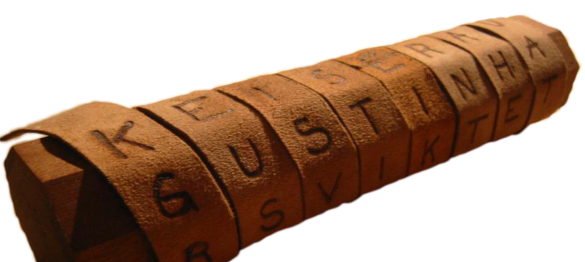
\includegraphics[width=64.05mm,height=72.17mm]{../../images/llm/page_049_img_01.png}%
\end{textblock*}

% deskripsi: Foto alat enkripsi cakram alfabet (cipher disk) yang digunakan untuk metode Caesar cipher.
% bbox normalisasi: [0.0600, 0.1080, 0.9400, 0.9120]
\begin{textblock*}{184.80mm}(12.60mm,32.08mm)
\noindent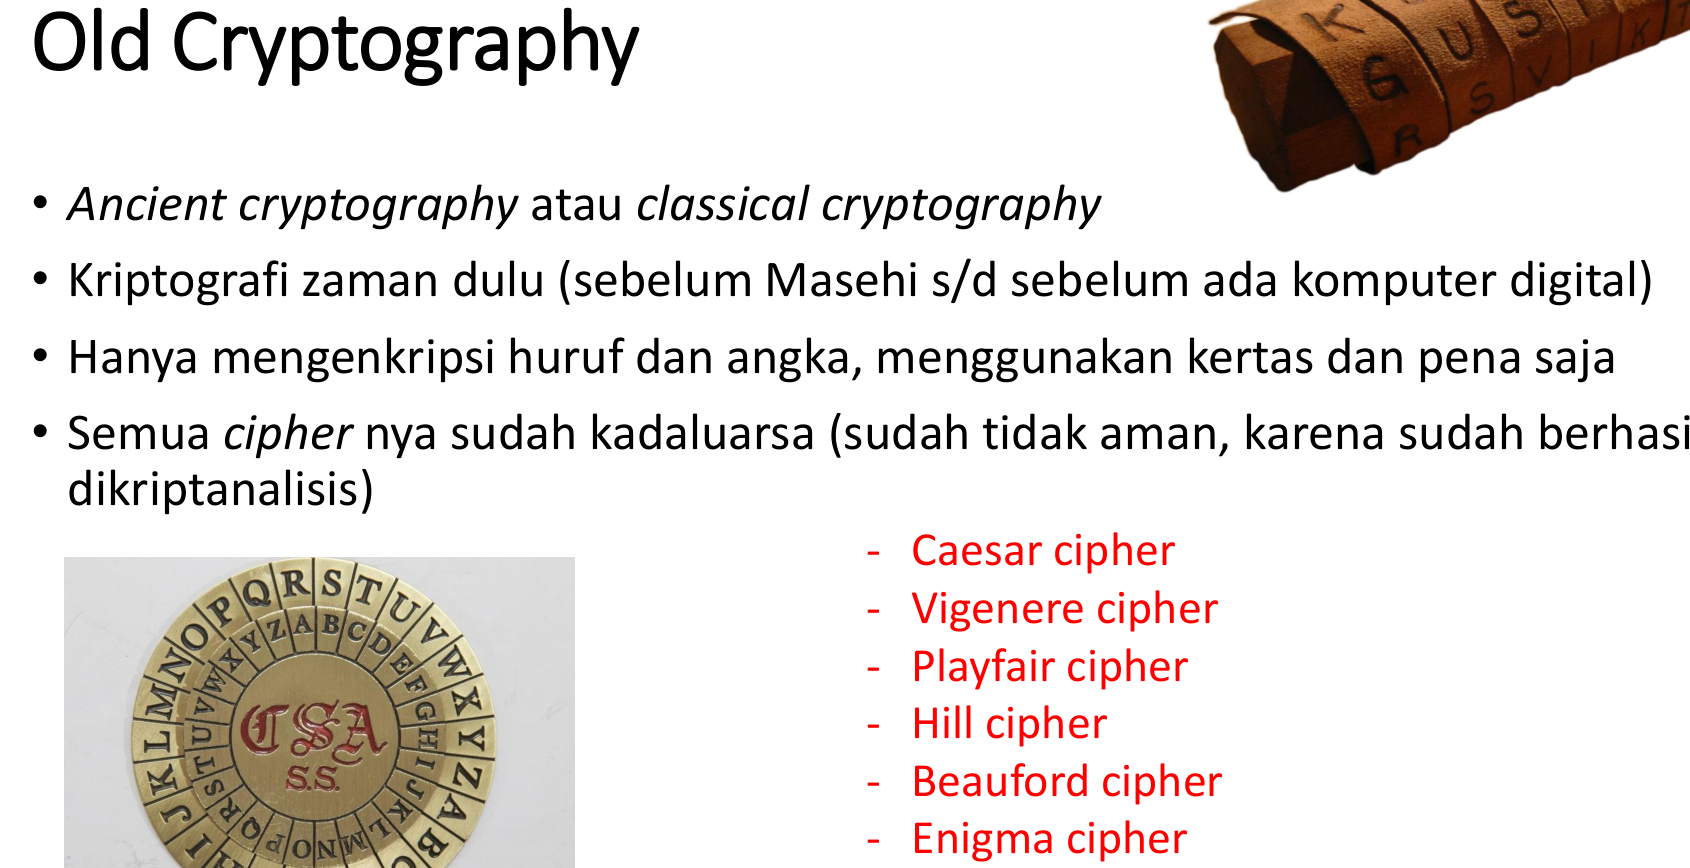
\includegraphics[width=184.80mm,height=238.79mm]{../../images/llm/page_049_img_02.png}%
\end{textblock*}

% bbox perkiraan otomatis: Foto alat enkripsi cakram alfabet (cipher disk) yang digunakan untuk metode Caesar cipher.

\end{document}
